% DM d'optimisation (CentraleSupélec) -- décodage spéculatif -- VERSION COURTE
% Compilation : pdflatex rapport_dm_court.tex (deux passes pour les références croisées)
% La version complète (preuves détaillées, exemples, validation) est rapport_dm.tex.
\documentclass[11pt,a4paper]{article}
\usepackage[utf8]{inputenc}
\usepackage[T1]{fontenc}
\usepackage{lmodern}
\usepackage[french]{babel}
\frenchsetup{SmallCapsFigTabCaptions=false,og=«,fg=»}
\usepackage[a4paper,margin=2.2cm]{geometry}
\usepackage{amsmath,amssymb,amsthm,mathtools}
\usepackage{graphicx}
\usepackage{booktabs,tabularx,array}
\usepackage{enumitem}
\usepackage[dvipsnames]{xcolor}
\usepackage{microtype}
\usepackage{caption}
\usepackage[colorlinks=true,linkcolor=MidnightBlue,citecolor=MidnightBlue,urlcolor=MidnightBlue]{hyperref}
\usepackage{xurl}

\captionsetup{font=small,labelfont=bf,format=hang,justification=justified}
\setlist{itemsep=2pt,topsep=3pt}
\setlength{\parskip}{3pt}
\graphicspath{{figures/}}

\newcommand{\R}{\mathbb{R}}
\newcommand{\TV}{\mathrm{TV}}
\newcommand{\Prob}{\mathbb{P}}
\newcommand{\Esp}{\mathbb{E}}
\newcommand{\sca}[2]{\langle #1,#2\rangle}
\newcommand{\nr}[1]{\|#1\|}
\newcommand{\clip}{\operatorname{clip}}
\newcommand{\vecop}{\operatorname{vec}}
\newcommand{\diag}{\operatorname{diag}}
\newcommand{\rg}{\operatorname{rg}}
\newcommand{\cB}{\mathcal{B}}
\newcommand{\cN}{\mathcal{N}}
\newcommand{\tok}[1]{\texttt{#1}}

\theoremstyle{plain}
\newtheorem{proposition}{Proposition}
\newtheorem{lemme}{Lemme}

\title{\textbf{Où relâcher la vérification ?}\\[2pt]
\large Allocation optimale d'un budget de déviation en décodage spéculatif}
\author{Prénom~Nom~1 \and Prénom~Nom~2\\[2pt]
\small DM d'optimisation, CentraleSupélec, dominante Mathématiques et Sciences des Données, 2026--2027}
\date{}

\begin{document}
\maketitle

\begin{abstract}
En décodage spéculatif, un petit modèle (le \emph{draft}) propose des tokens qu'un grand modèle (le \emph{target}) vérifie en une seule passe.
\textbf{(I)} Vérifier un token est un programme linéaire de transport : notre simplexe et un certificat dual explicite montrent que l'acceptation maximale vaut $1-\TV(p,q)$ ; tolérer une déviation $\varepsilon$ de la loi émise la porte à $\min(1,1-\TV+\varepsilon)$, avec un prix dual de~1.
\textbf{(II)} Répartir un budget de déviation entre les positions d'un bloc drafté est un problème \emph{non concave} sous contraintes linéaires, que nous traitons par les conditions KKT et le gradient projeté.
Comme un rejet termine le bloc, le budget doit aller d'abord aux \textbf{premières} positions, même plus sensibles : dans un scénario typique, l'allocation optimale est 26\,\% plus rapide qu'un modèle qui ignore cette structure.
\end{abstract}

\begin{center}
\small
\begin{tabularx}{\linewidth}{@{}>{\raggedright}p{0.36\linewidth}X@{}}
\toprule
\textbf{Attendu du DM} & \textbf{Où} \\\midrule
Modélisation & §\ref{sec:modeleI} (PL), §\ref{sec:modeleII} (allocation)\\
Existence et unicité & §\ref{sec:existenceI} (PL : non-unicité caractérisée), §\ref{sec:existenceII} (non-concavité, cas $\gamma=2$)\\
Théorèmes du cours, conditions d'optimalité & dualité en PL (§\ref{sec:dualite}), KKT, Th.~2.5.17 (§\ref{sec:kkt}), Euler, Th.~2.5.1 (annexe~\ref{app:convergence})\\
Algorithme et convergence & simplexe en deux phases (§\ref{sec:simplexe}), gradient projeté (§\ref{sec:algoII}, annexe~\ref{app:convergence})\\
Plusieurs minima locaux ? & objectif non concave, multi-départs (§\ref{sec:algoII})\\
Originalité & \textbf{méthode du simplexe}, \textbf{mise en œuvre de la dualité} (certificat, prix duaux)\\
\bottomrule
\end{tabularx}
\end{center}

%=====================================================================
\section{Contexte et notations}\label{sec:contexte}
%=====================================================================
À chaque position, le target définit une loi $p$ sur le vocabulaire et le draft une loi $q$.
La règle de Leviathan et al.~\cite{leviathan} (proposée indépendamment par Chen et al.~\cite{chen}) accepte le token drafté $x\sim q$ avec probabilité $\min(1,p_x/q_x)$ ; en cas de rejet, elle ré-échantillonne dans $(p-q)_+$ normalisée, et la loi émise est alors exactement $p$.
Le draft propose un bloc de $\gamma$ tokens, que le target vérifie en \emph{une} passe ; le premier rejet termine le bloc, et la vitesse se mesure par le nombre moyen de tokens produits par passe du target.
On note $\TV(p,q)=\tfrac12\nr{p-q}_1$ et $\beta(p,q)=\sum_i\min(p_i,q_i)=1-\TV(p,q)$.

Une vérification \emph{avec perte}~\cite{fuzzy} accepte plus souvent, au prix d'une déformation de la loi émise.
Sur GSM8K, avec Qwen2.5-0.5B comme draft et Qwen2.5-1.5B comme target, la plupart des rejets portent sur des \textbf{synonymes} sans effet sur la réponse (\tok{determine} contre \tok{find}), et quelques-uns sur des \textbf{pivots} qui orientent le raisonnement (\tok{not} contre \tok{left}, c'est-à-dire « ce qui est utilisé » contre « ce qui reste »).
Relâcher la vérification sur les premiers fait gagner de la vitesse sans risque ; sur les seconds, il ne faut pas. Ce DM formalise ce compromis.

%=====================================================================
\section{Partie I : vérifier un token est un programme linéaire}
%=====================================================================
\subsection{Modèle}\label{sec:modeleI}
Une règle de vérification (exacte ou non) est décrite par la loi jointe du couple (token proposé, token émis) : $\pi\in\R_+^{n\times n}$, $\pi_{xy}=\Prob(\text{le draft propose }x\text{ et l'on émet }y)$. On accepte exactement quand $y=x$ : l'acceptation est la trace de $\pi$. Le draft propose selon $q$ (lignes) et la règle est exacte si le token émis suit $p$ (colonnes) :
\[(P_0)\qquad \max_{\pi\ge0}\ \sum_x\pi_{xx}\quad\text{s.c.}\quad \sum_y\pi_{xy}=q_x\ \ (x=1,\dots,n),\qquad \sum_x\pi_{xy}=p_y\ \ (y=1,\dots,n).\]
En forme standard ($\min c\cdot x$, $Ax=b$, $x\ge0$), $c=-\vecop(I_n)$, $b=(q,p)\in\R^{2n}$, et $A\in\{0,1\}^{2n\times n^2}$ a une colonne par variable $\pi_{xy}$, avec un 1 sur la ligne $x$ et un 1 sur la ligne $n+y$.
\begin{itemize}
\item \textbf{Flot.} En multipliant par $-1$ les $n$ lignes « colonne », chaque colonne de $A$ a un $+1$ et un $-1$ : c'est la matrice d'incidence d'un graphe biparti orienté, totalement unimodulaire par le lemme de Poincaré (Lemme~4.3.5) ; changer le signe d'une ligne ne change que des signes de déterminants, donc $A$ est TU. Comme $b$ n'est pas entier, cela ne sert pas à l'intégrité, mais situe $(P_0)$ parmi les problèmes de flot du cours.
\item \textbf{Rang.} Les $n$ lignes du haut et les $n$ lignes du bas ont la même somme $(1,\dots,1)$, donc $\rg(A)\le2n-1$ ; sans la ligne « colonne 1 », les colonnes de $\pi_{11}$, des $\pi_{1y}$ ($y\ge2$) et des $\pi_{x1}$ ($x\ge2$) engendrent $\R^{2n-1}$, donc $\rg(A)=2n-1$. Le cours supposant $A$ de rang plein, le code retire une ligne avant le simplexe.
\item \textbf{Compatibilité.} Le système exige $\sum_xq_x=\sum_yp_y$ ; les lois réelles (sommes $1\pm10^{-6}$ en float32) sont donc renormalisées.
\end{itemize}

\subsection{Existence, valeur et (non-)unicité}\label{sec:existenceI}
L'ensemble admissible est non vide (couplage indépendant $\pi_{xy}=q_xp_y$) et borné ($0\le\pi_{xy}\le q_x$) : c'est un polyèdre compact, et le maximum de l'objectif linéaire est atteint (Th.~2.2.1), en un sommet (Prop.~4.2.6).

\begin{proposition}[valeur de $(P_0)$]\label{prop:valeur}
La valeur de $(P_0)$ vaut $\beta(p,q)=1-\TV(p,q)$. Les solutions optimales sont exactement les $\pi\ge0$ telles que $\pi_{xx}=\min(p_x,q_x)$ et dont la partie hors diagonale a pour marges $(q-p)_+$ (lignes) et $(p-q)_+$ (colonnes). La solution est unique si et seulement si l'un de ces deux vecteurs a au plus une composante non nulle.
\end{proposition}
On utilise $\min(a,b)+(a-b)_+=a$ et $\sum_x(p_x-q_x)_+=\sum_x(q_x-p_x)_+=\TV$ (leur différence vaut $\sum_x(p_x-q_x)=0$, leur somme $2\,\TV$), d'où $\beta=\sum_x\big(p_x-(p_x-q_x)_+\big)=1-\TV$.
\begin{proof}
\emph{Majoration.} Une case diagonale est majorée par la somme de sa ligne et par celle de sa colonne : $\pi_{xx}\le\min(p_x,q_x)$, donc $\sum_x\pi_{xx}\le\beta$.

\emph{Borne atteinte.} Si $\TV=0$, $\diag(p)$ convient. Sinon, la règle de~\cite{leviathan} induit le couplage
\[\pi^L=\diag\big(\min(p,q)\big)+\frac{(q-p)_+\,(p-q)_+^{\top}}{\TV}:\]
proposer $x$ et l'accepter a probabilité $q_x\min(1,p_x/q_x)=\min(p_x,q_x)$ ; proposer $x$ et le rejeter a probabilité $(q_x-p_x)_+$, puis $y$ est tiré selon $(p-q)_+/\TV$. Ses lignes valent $\min(p_x,q_x)+(q_x-p_x)_+=q_x$, ses colonnes $\min(p_y,q_y)+(p_y-q_y)_+=p_y$, et le terme de rang 1 est nul sur la diagonale ($(q_x-p_x)_+(p_x-q_x)_+=0$) : sa trace vaut $\beta$.

\emph{Toutes les solutions.} À l'optimum, les inégalités de la majoration sont des égalités : $\pi_{xx}=\min(p_x,q_x)$. Il reste $(q_x-p_x)_+$ à placer sur la ligne $x$ et $(p_y-q_y)_+$ sur la colonne $y$, et une case hors diagonale non nulle exige $q_x>p_x$ et $p_y>q_y$. Réciproquement, tout $\pi\ge0$ de cette forme est admissible et de trace $\beta$.

\emph{Unicité.} Supposons que $\{q>p\}$ et $\{p>q\}$ aient chacun au moins deux éléments. Chaque colonne de $\{p>q\}$ reçoit une masse $>0$, d'où $\pi_{x_1y_1}>0$ et $\pi_{x_2y_2}>0$ avec $y_1\ne y_2$ ; si $x_1=x_2$, une autre ligne $x'\in\{q>p\}$ a une case $\pi_{x'y''}>0$, avec $y''$ différent de $y_1$ ou de $y_2$. On dispose ainsi de $\pi_{xy}>0$ et $\pi_{x'y'}>0$ avec $x\ne x'$, $y\ne y'$. Retirer $\delta\in\,]0,\min(\pi_{xy},\pi_{x'y'})]$ à ces deux cases et l'ajouter à $\pi_{xy'}$ et $\pi_{x'y}$ conserve les marges et la diagonale (les quatre cases sont hors diagonale, car $\{q>p\}\cap\{p>q\}=\emptyset$) : c'est une autre solution optimale. Si l'un des deux ensembles a au plus un élément, la partie hors diagonale est forcée, et la solution est unique.
\end{proof}

\subsection{Dualité : un certificat d'optimalité explicite}\label{sec:dualite}
Le dual de $\min\{c\cdot x:Ax=b,\ x\ge0\}$ est $\max\{b\cdot\mu:A^\top\mu\le c\}$ (Th.~4.2.13). Avec $\mu=(\varphi,\psi)$ (multiplicateurs des lignes et des colonnes), $(A^\top\mu)_{xy}=\varphi_x+\psi_y$ et $c_{xy}=-\delta_{xy}$ :
\[(D_0)\qquad \max_{\varphi,\psi}\ q\cdot\varphi+p\cdot\psi\quad\text{s.c.}\quad \varphi_x+\psi_y\le-\delta_{xy}\quad\forall x,y.\]
Pour $\pi$ et $\mu$ admissibles, $c\cdot\pi\ge(A^\top\mu)\cdot\pi=\mu\cdot b$ (dualité faible) : une égalité certifie l'optimalité des deux.
Posons $S=\{x:q_x\le p_x\}$, $\varphi_x=-1$ si $x\in S$ et $0$ sinon, $\psi_y=0$ si $y\in S$ et $-1$ sinon. Sur la diagonale, exactement l'un des deux vaut $-1$, donc $\varphi_x+\psi_x=-1$ ; hors diagonale, $\varphi_x+\psi_y\le0$ : $(\varphi,\psi)$ est admissible, de valeur $-\sum_{x\in S}q_x-\sum_{y\notin S}p_y=-\beta=c\cdot\pi^L$. Les deux sont donc optimaux, ce qui redémontre la proposition~\ref{prop:valeur}.
Les écarts complémentaires ($\pi_{xy}>0\Rightarrow\varphi_x+\psi_y=c_{xy}$) se vérifient sur $\pi^L$ : une case hors diagonale non nulle a $q_x>p_x$ et $p_y>q_y$, donc $\varphi_x+\psi_y=0=c_{xy}$. \emph{Lecture :} $\varphi_x=-1$ marque les tokens que le draft propose « trop peu » ($q_x\le p_x$), toujours acceptés.

\subsection{Simplexe révisé en deux phases, et validation}\label{sec:simplexe}
Le simplexe est programmé comme dans le cours. Avec la base $\cB$ et les hors-base $\cN$ : $x_\cB=A_\cB^{-1}b$, multiplicateurs $\mu=A_\cB^{-\top}c_\cB$, coûts réduits $\tilde c_\cN=c_\cN-A_\cN^\top\mu$ ; si $\tilde c_\cN\ge0$, la base est optimale (Prop.~4.2.8) ; sinon, la variable de coût réduit le plus négatif entre, et le test du ratio $\theta^*=\min\{x_{\cB,i}/d_i:d_i>0\}$, avec $d=A_\cB^{-1}A_j$, désigne la variable sortante. La phase~1 (variables artificielles) fournit une base admissible, ou prouve que le problème ne l'est pas. Les bases sont très dégénérées ($2n-1$ variables de base, souvent nulles) : pour exclure le cyclage, on passe à la règle de Bland après $2m$ pivots dégénérés consécutifs ($m=2n-1$ contraintes). Les multiplicateurs de la base finale donnent le dual (§\ref{sec:perte}).

\textbf{Validation.} Sur 300 paires synthétiques ($n=3$ à $12$, lois de Dirichlet plus ou moins piquées), notre simplexe, le solveur HiGHS de SciPy et la formule $\beta$ coïncident à $4{,}4\times10^{-16}$ près ; sur 320 paires réelles (Qwen2.5, réduites aux 6 tokens les plus probables de chaque modèle plus une case « autres »), à $3{,}5\times10^{-11}$ près, au niveau de la tolérance du test d'optimalité (figure~\ref{fig:lp}a). Des tests unitaires vérifient l'admissibilité duale, la dualité forte et le certificat $(\varphi,\psi)$. Le nombre d'itérations croît environ comme $n^{1{,}7}$ : pour un vrai vocabulaire ($n\approx150\,000$, plus de $2\times10^{10}$ variables), on utilise la formule fermée, que le simplexe sert à valider. Enfin, le simplexe renvoie un sommet (8 cases non nulles, au plus $2n-1=9$) et $\pi^L$ en a 11 : deux optimums distincts, comme le prévoit la proposition~\ref{prop:valeur} (figure~\ref{fig:lp}b-c).

\begin{figure}[htbp]
\centering
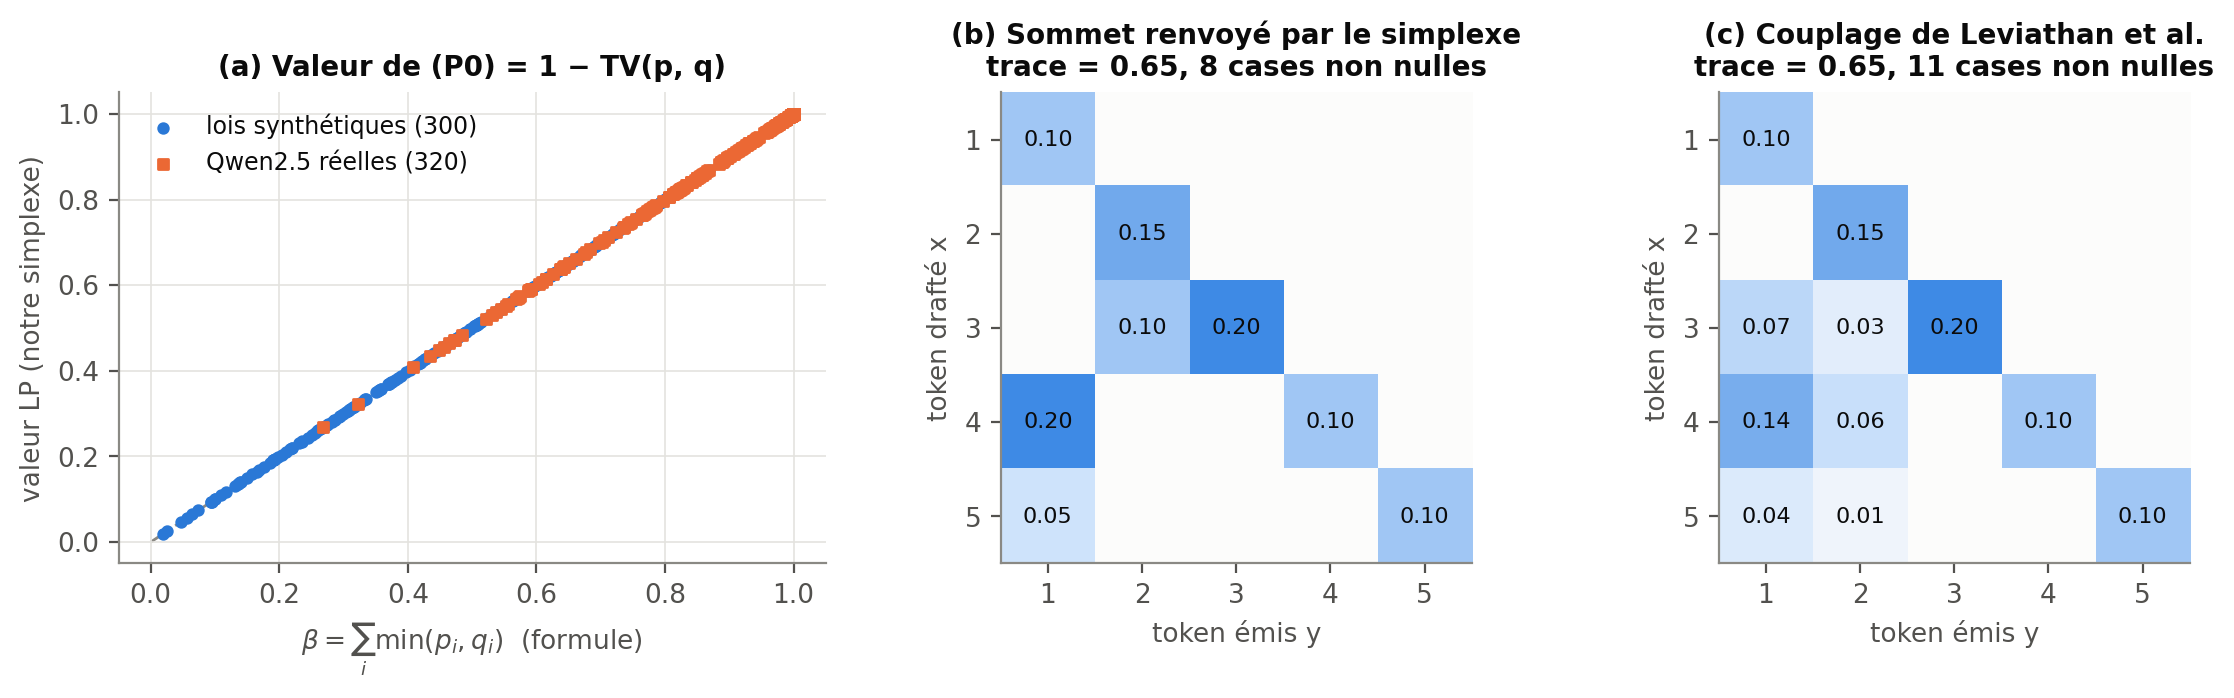
\includegraphics[width=0.94\linewidth]{fig1_lp_exact.png}
\caption{(a) Valeur de $(P_0)$ calculée par notre simplexe contre la formule $\beta=\sum\min(p,q)$. (b-c) Deux couplages optimaux pour $p=(0{,}35;0{,}25;0{,}2;0{,}1;0{,}1)$ et $q=(0{,}1;0{,}15;0{,}3;0{,}3;0{,}15)$ : même diagonale, partie hors diagonale différente.}
\label{fig:lp}
\end{figure}

\subsection{Vérification avec perte et prix dual du budget}\label{sec:perte}
On autorise la loi émise $r$ à s'écarter de $p$ d'au plus $\varepsilon$ en variation totale : la seconde marge de $\pi$ devient une variable $r$ (automatiquement une loi), et l'on linéarise $|r_y-p_y|$ par $t_y\ge\pm(r_y-p_y)$ (le choix $t_y=|r_y-p_y|$ montre que les deux formulations ont les mêmes $(\pi,r)$ admissibles) :
\[(P_\varepsilon)\qquad \max_{\pi,r,t\ge0}\ \sum_x\pi_{xx}\quad\text{s.c.}\quad \textstyle\sum_y\pi_{xy}=q_x,\quad \sum_x\pi_{xy}=r_y,\quad t_y\ge\pm(r_y-p_y),\quad \sum_yt_y\le2\varepsilon.\]

\begin{proposition}[frontière avec perte]\label{prop:perte}
La valeur de $(P_\varepsilon)$ vaut $\alpha^*(\varepsilon)=\min(1,\beta+\varepsilon)$, atteinte pour $r_\varepsilon=p+\theta(q-p)$, $\theta=\min(1,\varepsilon/\TV)$.
\end{proposition}
\begin{proof}
Pour $(\pi,r,t)$ admissible, $\pi$ couple $q$ et $r$ : par la proposition~\ref{prop:valeur} et l'inégalité triangulaire, $\sum_x\pi_{xx}\le1-\TV(q,r)\le1-\TV(q,p)+\TV(r,p)\le\beta+\varepsilon$, et $\sum_x\pi_{xx}\le1$. Inversement, $\TV(r_\varepsilon,p)=\theta\,\TV\le\varepsilon$ et $\TV(q,r_\varepsilon)=(1-\theta)\TV$ : le couplage de Leviathan entre $q$ et $r_\varepsilon$ accepte avec probabilité $\beta+\theta\,\TV=\min(1,\beta+\varepsilon)$.
\end{proof}

\paragraph{Le multiplicateur du budget est une pente.} Soit $V(\varepsilon)=-\alpha^*(\varepsilon)$ la valeur en minimisation. L'ensemble dual $D=\{\mu:A^\top\mu\le c\}$ ne dépend pas de $\varepsilon$ ; seul le second membre $b(\varepsilon)=b_0+2\varepsilon\,e_{\text{budget}}$ en dépend. Par dualité forte, $V(\varepsilon)=\max_{\mu\in D}b(\varepsilon)\cdot\mu$ est convexe et, pour un dual optimal $\mu^*$ en $\varepsilon$, $V(\varepsilon')\ge b(\varepsilon')\cdot\mu^*=V(\varepsilon)+2\mu^*_B(\varepsilon'-\varepsilon)$. Le \textbf{prix du budget} $\kappa=-2\mu^*_B\ge0$ ($\mu^*_B\le0$, car l'écart de la ligne de budget a un coût nul) est donc un sur-gradient de $\alpha^*$ : le gain d'acceptation par unité de déviation. Il vaut 1 pour $\varepsilon<\TV$ et 0 au-delà, ce que renvoie le simplexe (figure~\ref{fig:perte}b) ; aux coins, il n'est pas unique (tout $\kappa\in[0,1]$ en $\varepsilon=\TV$, tout $\kappa\ge1$ en $\varepsilon=0$). \textbf{Une unité de déviation achète exactement une unité d'acceptation} tant qu'il reste du désaccord : c'est la frontière linéaire de~\cite{yin}, retrouvée avec les outils du cours, et la brique de la partie II.

\begin{figure}[htbp]
\centering
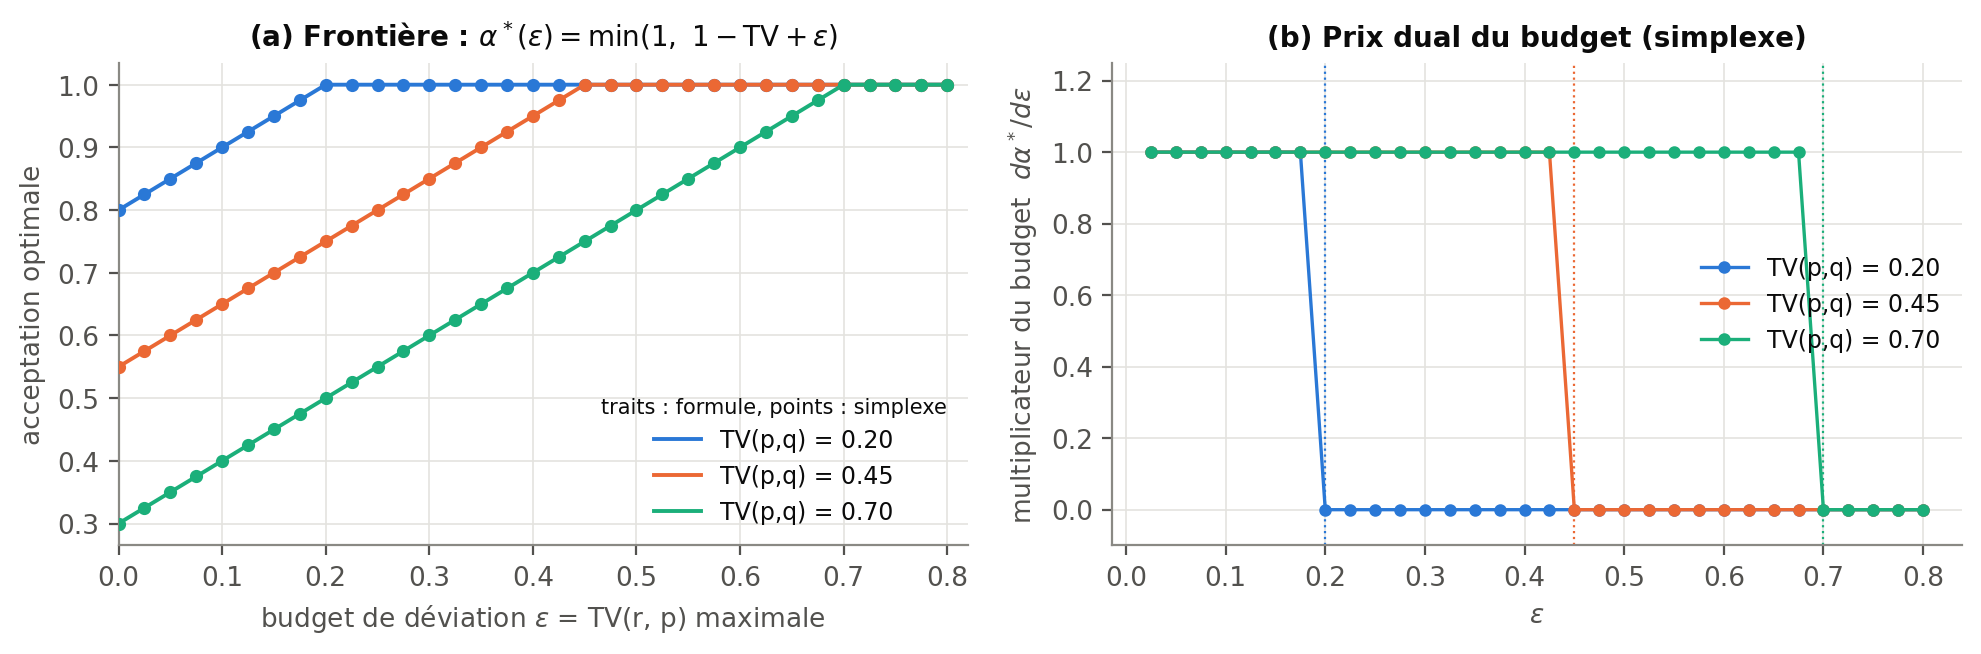
\includegraphics[width=0.86\linewidth]{fig2_lossy_frontier.png}
\caption{(a) Acceptation optimale en fonction de $\varepsilon$ pour trois paires $(p,q)$ ; points : simplexe, traits : proposition~\ref{prop:perte}. (b) Prix du budget $\kappa=-2\mu^*_B=d\alpha^*/d\varepsilon$ tiré du dual renvoyé par le simplexe : 1 avant $\varepsilon=\TV$ (pointillés), 0 après.}
\label{fig:perte}
\end{figure}

%=====================================================================
\section{Partie II : répartir le budget entre les positions d'un bloc}
%=====================================================================
\subsection{Modèle}\label{sec:modeleII}
Un bloc compte $\gamma$ positions. La position $t$ a une acceptation exacte $a_t=\beta(p_t,q_t)\in(0,1)$ et une \textbf{sensibilité} $s_t>0$ (baisse de qualité de la réponse par unité de déviation). Les variables sont les déviations $\varepsilon\in\R^\gamma$, sous trois hypothèses : (H1) acceptations indépendantes, comme dans~\cite{leviathan} ; (H2) perte de qualité additive, $\sum_ts_t\varepsilon_t$ ; (H3) par la proposition~\ref{prop:perte}, relâcher la position $t$ de $\varepsilon_t$ donne l'acceptation $\alpha_t=a_t+\varepsilon_t$, avec $0\le\varepsilon_t\le u_t:=1-a_t$ (la \emph{marge}).

Le bloc s'arrête au premier rejet : « au moins $k$ acceptés » signifie « les $k$ premiers acceptés », de probabilité $P_k=\alpha_1\cdots\alpha_k$ ($P_0=1$). Avec $\Esp[N]=\sum_{k\ge1}\Prob(N\ge k)$ et le token que le target émet à la fin de chaque passe, le nombre moyen de tokens par passe vaut
\[E(\varepsilon)=1+\sum_{k=1}^{\gamma}\prod_{j=1}^{k}(a_j+\varepsilon_j),\qquad (Q_B)\quad \max_{\varepsilon\in K}E(\varepsilon),\quad K=\{0\le\varepsilon\le u,\ s\cdot\varepsilon\le B\}.\]
Les contraintes sont affines. On compare au \textbf{modèle A}, qui ignore la structure en bloc et maximise $\sum_t\alpha_t$ (un sac à dos fractionnaire).

\subsection{Existence et structure}\label{sec:existenceII}
$K$ est un polyèdre non vide ($0\in K$) et compact, $E$ est continue : un maximum existe (Th.~2.2.1).
$\alpha_t$ n'apparaît, linéairement, que dans les $P_k$ avec $k\ge t$, d'où
\[\partial_tE=P_{t-1}\,T_t>0,\qquad T_t=1+\alpha_{t+1}+\alpha_{t+1}\alpha_{t+2}+\dots+\alpha_{t+1}\cdots\alpha_\gamma,\]
produit de la \textbf{probabilité d'atteindre} la position $t$ et du \textbf{nombre de tokens} que son acceptation débloque.
$E$ est affine en chaque variable, donc $\partial^2_{tt}E=0$, et pour $i<j$, $\partial^2_{ij}E=P_{i-1}\big(\prod_{i<k<j}\alpha_k\big)T_j>0$. La hessienne, symétrique, non nulle et de trace nulle, a une valeur propre $>0$ en tout point : \textbf{$E$ n'est pas concave}, et les résultats d'unicité par convexité (Prop.~2.3.4, Th.~2.3.8) ne s'appliquent pas. Les dérivées croisées positives rendent les positions \textbf{complémentaires} : relâcher l'une fait atteindre plus souvent les suivantes.

\begin{lemme}[concavité le long des échanges]\label{lem:echange}
Pour $i\ne j$, la direction $d=s_je_i-s_ie_j$ conserve le coût, et $h\mapsto E(\varepsilon+hd)$ est un trinôme strictement concave.
\end{lemme}
\begin{proof}
À autres coordonnées fixées, $E=c_0+c_i\alpha_i+c_j\alpha_j+\partial^2_{ij}E\,\alpha_i\alpha_j$ ; le long de $d$, le coefficient de $h^2$ vaut $-s_is_j\,\partial^2_{ij}E<0$.
\end{proof}
La non-concavité vient donc des directions qui font varier plusieurs positions dans le même sens.

\begin{lemme}[budget saturé]\label{lem:sature}
En tout maximum local, $s\cdot\varepsilon=B$, ou bien $\varepsilon=u$ (budget surabondant).
\end{lemme}
\begin{proof}
Si $s\cdot\varepsilon<B$ et $\varepsilon_t<u_t$, augmenter $\varepsilon_t$ reste admissible et augmente $E$, car $\partial_tE>0$.
\end{proof}

\begin{proposition}[cas $\gamma=2$ : unicité et solution explicite]\label{prop:gamma2}
Si $B<s\cdot u$, le maximum est unique. Avec $\kappa_s=s_1/s_2$, $c=a_2+B/s_2$ et $\eta^*=\tfrac12\big((1+c)/\kappa_s-a_1\big)$, on a $\varepsilon_1^*=\mathrm{proj}_{[\eta_-,\eta_+]}(\eta^*)$ et $\varepsilon_2^*=(B-s_1\varepsilon_1^*)/s_2$, où $[\eta_-,\eta_+]=\big[\max\big(0,(B-s_2u_2)/s_1\big),\min\big(u_1,B/s_1\big)\big]$. Si $\eta_-<\eta^*<\eta_+$,
\[E^*(B)=1+\frac{(1+c+\kappa_sa_1)^2}{4\kappa_s},\qquad \lambda^*=\frac{1+c+\kappa_sa_1}{2s_1}=\frac{dE^*}{dB}.\]
\end{proposition}
\begin{proof}
Par le lemme~\ref{lem:sature}, le maximum est sur le segment $s\cdot\varepsilon=B$. Avec $\varepsilon_1=\eta$, on a $\alpha_1=a_1+\eta$ et $\alpha_2=c-\kappa_s\eta$, d'où $E(\eta)=1+(a_1+\eta)(1+c-\kappa_s\eta)$, un trinôme strictement concave ($E''=-2\kappa_s$, c'est le lemme~\ref{lem:echange}) : son maximum sur $[\eta_-,\eta_+]$ est unique, égal à $\eta^*$ projeté. Si $\eta^*$ est intérieur, on obtient $E^*$, et $dc/dB=1/s_2$ donne $dE^*/dB=(1+c+\kappa_sa_1)/(2s_1)=(1+\alpha^*_2)/s_1=\partial_1E/s_1=\lambda^*$ (§\ref{sec:kkt}).
\end{proof}

\begin{proposition}[positions identiques : relâcher d'abord le début]\label{prop:ordre}
Si $a_t\equiv a$ et $s_t\equiv s$, toute solution optimale vérifie $\alpha_1\ge\alpha_2\ge\dots\ge\alpha_\gamma$.
\end{proposition}
\begin{proof}
Si $\alpha_t<\alpha_{t+1}$ à l'optimum, échanger $\varepsilon_t$ et $\varepsilon_{t+1}$ reste admissible ; seul $P_t=P_{t-1}\alpha_t$ change (les $P_k$, $k>t$, contiennent le produit $\alpha_t\alpha_{t+1}$), et $E$ augmente de $P_{t-1}(\alpha_{t+1}-\alpha_t)>0$ : contradiction.
\end{proof}

\begin{figure}[htbp]
\centering
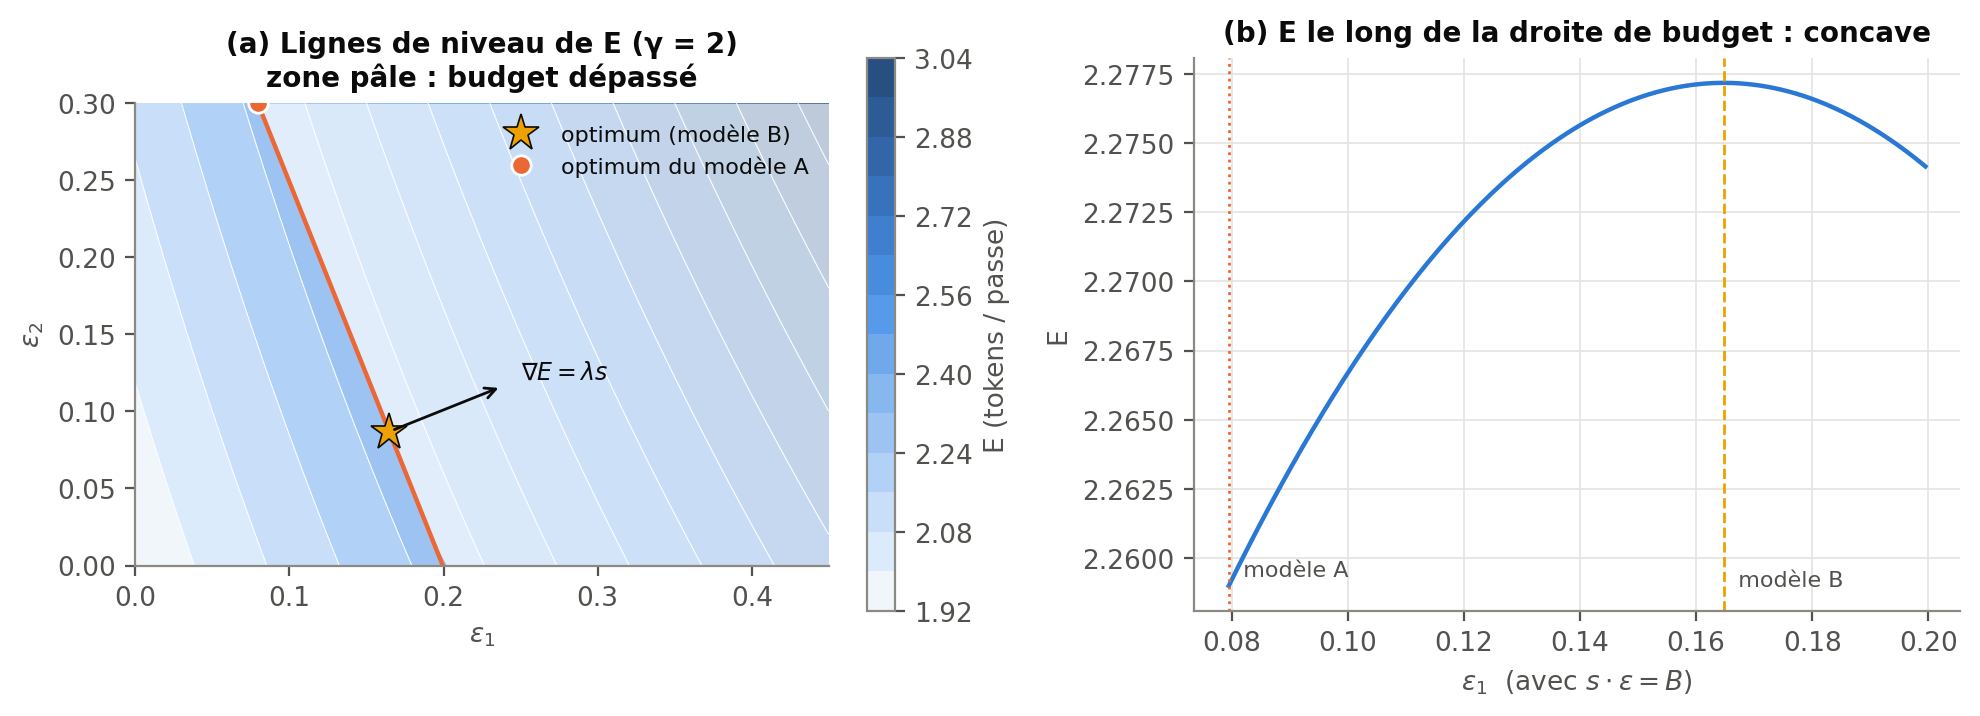
\includegraphics[width=0.8\linewidth]{fig3_landscape_gamma2.png}
\caption{$\gamma=2$, $a=(0{,}55;0{,}7)$, $s=(1{,}5;0{,}6)$, $B=0{,}35\,s\cdot u$. (a) À l'optimum $\varepsilon^*=(0{,}165;0{,}087)$, $\nabla E=\lambda s$ avec $\lambda=1{,}191=dE^*/dB$. (b) Le long de la droite de budget, $E$ est un trinôme concave ($E''=-5$) : $E^*=2{,}277$ (proposition~\ref{prop:gamma2}, retrouvé par le gradient projeté), contre $2{,}259$ pour le modèle A, qui choisit le bord.}
\label{fig:paysage}
\end{figure}

\subsection{Conditions d'optimalité (KKT)}\label{sec:kkt}
Les contraintes s'écrivent $F_i(\varepsilon)\le0$ : budget $s\cdot\varepsilon-B$ (multiplicateur $\lambda$), bornes $-\varepsilon_t$ et $\varepsilon_t-u_t$ (multiplicateurs $\mu^0_t,\mu^1_t$). Elles sont affines, donc qualifiées en tout point : la définition~2.5.15 autorise l'égalité $\sca{\nabla F_i}{w}=0$ pour les contraintes affines, et $w=0$ convient (Rq.~2.5.16). Le Th.~2.5.17, appliqué à $J=-E$, donne en tout maximum local de $E$ des $\lambda,\mu^0,\mu^1\ge0$ tels que
\[\nabla E(\varepsilon)=\lambda s-\mu^0+\mu^1,\qquad \lambda(s\cdot\varepsilon-B)=0,\quad \mu^0_t\varepsilon_t=0,\quad \mu^1_t(u_t-\varepsilon_t)=0.\]
Ces conditions sont \textbf{seulement nécessaires} : $J$ n'est pas convexe, donc le théorème de Kuhn--Tucker (Th.~2.6.4) ne s'applique pas.

\paragraph{Règle de seuil.} Avec le \textbf{rendement} $\rho_t=\partial_tE/s_t$ (tokens gagnés par unité de qualité perdue) : $\rho_t=\lambda$ si $0<\varepsilon_t<u_t$, $\rho_t\le\lambda$ si $\varepsilon_t=0$, $\rho_t\ge\lambda$ si $\varepsilon_t=u_t$. On relâche les positions dont le rendement dépasse le prix $\lambda$. Pour le modèle A, $\rho_t=1/s_t$ : on sature les positions par sensibilité croissante (sac à dos). Pour le modèle B, $\rho_t=P_{t-1}T_t/s_t$ dépend de la \textbf{place} : une position précoce est atteinte souvent et débloque beaucoup de tokens. C'est pourquoi le budget va au début du bloc.

\paragraph{$\lambda$ est le prix marginal du budget.} Soit $\varepsilon^*$ optimal pour $B$, avec une position intérieure $t$, et $0<h\le s_t\min(\varepsilon^*_t,u_t-\varepsilon^*_t)$. Les points $\varepsilon^*\pm(h/s_t)e_t$ sont admissibles pour les budgets $B\pm h$, et $E$, affine en $\varepsilon_t$, y vaut exactement $E^*(B)\pm\partial_tE\,h/s_t=E^*(B)\pm\lambda h$ (car $\rho_t=\lambda$). Donc $E^*(B\pm h)\ge E^*(B)\pm\lambda h$ :
\begin{equation}\label{eq:encadrement}
\frac{E^*(B)-E^*(B-h)}{h}\ \le\ \lambda\ \le\ \frac{E^*(B+h)-E^*(B)}{h}.
\end{equation}
Là où $E^*$ est dérivable, $\lambda=dE^*/dB$ : c'est l'analogue du lemme~2.6.6 du cours, qui suppose la convexité, obtenu ici grâce à la seule structure multilinéaire de $E$.

\subsection{Algorithme : gradient projeté, et question des maxima locaux}\label{sec:algoII}
On utilise le gradient projeté du cours, en montée : $\varepsilon_{k+1}=P_K\big(\varepsilon_k+\tau\nabla E(\varepsilon_k)\big)$.

\textbf{Projection.} $P_K(y)$ minimise $\tfrac12\nr{z-y}^2$, fortement convexe : elle existe et est unique (Th.~2.3.8). En dualisant le budget avec $\nu\ge0$, le problème se sépare et donne $z_t(\nu)=\clip(y_t-\nu s_t,0,u_t)$. On prend $\nu=0$ si $s\cdot z(0)\le B$ ; sinon, $\Phi(\nu)=s\cdot z(\nu)$ décroît continûment de $\Phi(0)>B$ à $0$, et une dichotomie trouve $\Phi(\nu)=B$. Avec les multiplicateurs des bornes $\omega^0_t=(\nu s_t-y_t)_+$ et $\omega^1_t=(y_t-\nu s_t-u_t)_+$, $(z(\nu),\nu,\omega^0,\omega^1)$ vérifie KKT pour ce problème convexe à contraintes affines, où ces conditions sont suffisantes (Th.~2.6.4) : $z(\nu)=P_K(y)$.

\textbf{Pas.} Sur $K$, $\alpha\in[0,1]^\gamma$ donne $|\partial^2_{ij}E|\le\gamma-\max(i,j)+1$ ; la norme de Frobenius majorant la norme de la hessienne, $\nabla E$ est $L$-lipschitzien sur $K$ avec
\[L=\Big(\sum_{i\ne j}\big(\gamma-\max(i,j)+1\big)^2\Big)^{1/2},\qquad\text{et l'on prend }\tau=1/L.\]

\textbf{Convergence.} Le Th.~3.4.1 suppose $J$ $\alpha$-convexe et ne s'applique pas, pas plus qu'Uzawa (Th.~3.4.3). On montre en annexe~\ref{app:convergence}, avec l'inéquation d'Euler, que $E(\varepsilon_k)$ croît, que les pas tendent vers 0 et que toute valeur d'adhérence vérifie KKT : c'est la meilleure garantie générale pour un problème non concave.

\textbf{Global ou local ?} Sur 100 instances aléatoires ($\gamma\in\{3,4,6,8\}$), 20 départs aléatoires chacune aboutissent à la même valeur, à $1{,}8\times10^{-15}$ près (résidu KKT $\le2{,}9\times10^{-10}$) : nous n'avons \textbf{jamais observé deux maxima locaux distincts}. Le problème est non concave mais, empiriquement, unimodal ; l'unicité n'est démontrée que pour $\gamma=2$.

\begin{figure}[htbp]
\centering
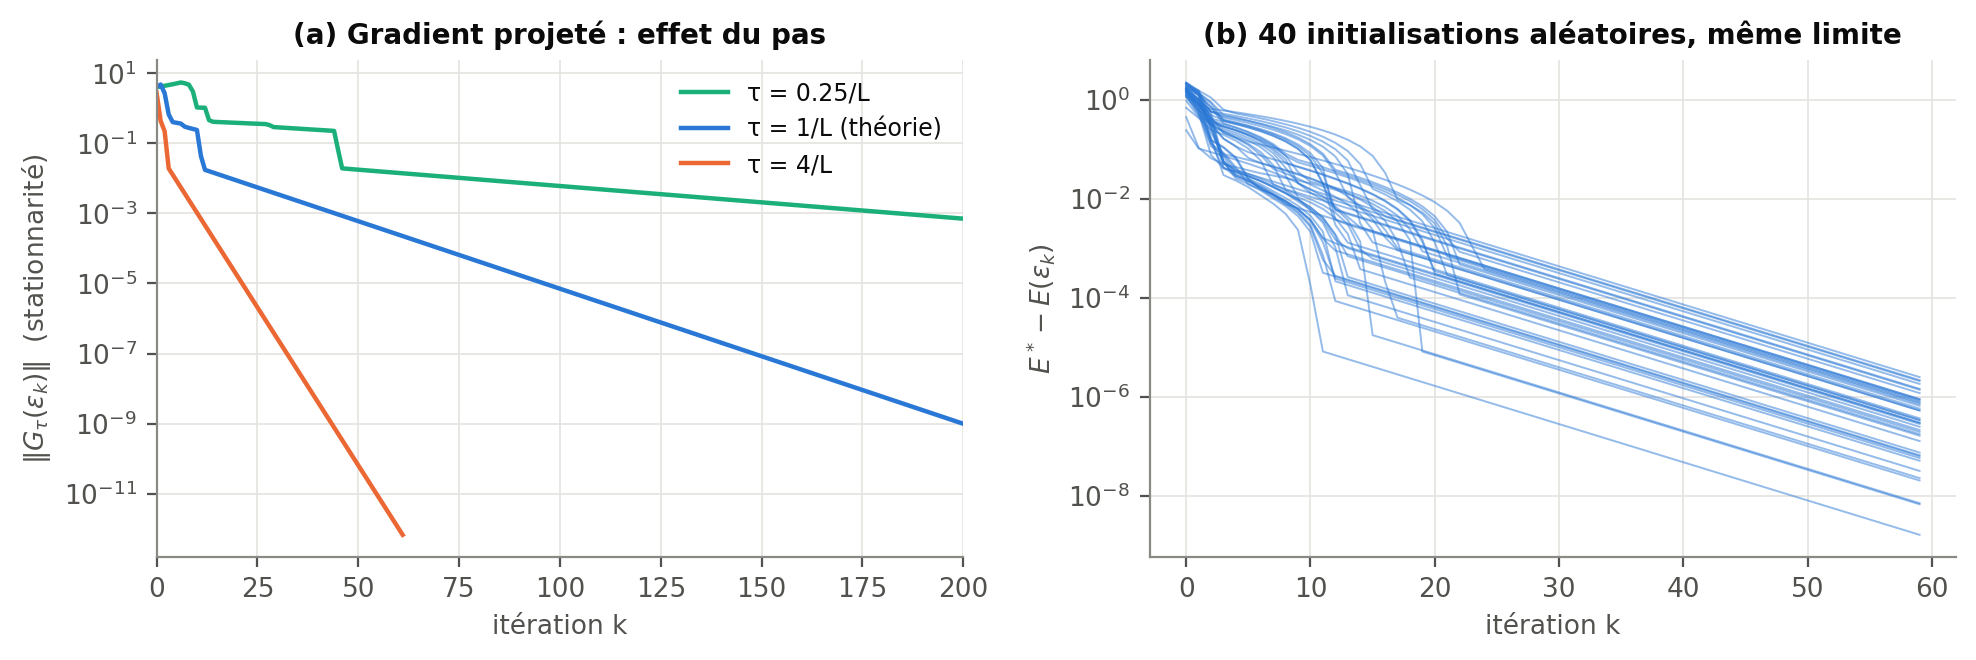
\includegraphics[width=0.8\linewidth]{fig4_convergence.png}
\caption{Instance $\gamma=8$. (a) Norme de l'application gradient : convergence linéaire, en 279 itérations pour $\tau=1/L$ (62 pour $\tau=4/L$, sans garantie de montée). (b) 40 départs aléatoires convergent vers la même valeur $E^*=5{,}4544$.}
\label{fig:convergence}
\end{figure}

\subsection{Résultats : où placer la déviation ?}\label{sec:resultats}
On prend $\gamma=6$, $a_t=0{,}6$, $B=0{,}3\,B_{\max}$ ($B_{\max}=s\cdot u$) et trois profils de sensibilité (figure~\ref{fig:allocation}).
\textbf{S1} ($s_t=1$) : B relâche dans l'ordre $1,2,\dots$ (proposition~\ref{prop:ordre}) ; A est indifférent entre toutes les répartitions de même coût, y compris « fin d'abord », qui ne donne que $E=2{,}54$ contre $4{,}12$.
\textbf{S2} (début plus sensible, $s=(2;1{,}7;1{,}4;1{,}1;0{,}8;0{,}5)$) : A relâche les dernières positions, les moins chères ; B relâche malgré tout les \textbf{premières}, avec $E=3{,}52$ contre $2{,}79$ pour A ($+26\,\%$) et $3{,}21$ pour une déviation uniforme ; à l'optimum, $\rho_1=\rho_2=\lambda=1{,}308$ et $\rho_t<\lambda$ ailleurs, comme le prévoit KKT.
\textbf{S3} (pivots coûteux en positions 2 et 5) : B évite le pivot tardif mais relâche en partie le pivot précoce, qui conditionne l'accès aux positions suivantes ($4{,}98$ contre $4{,}96$ pour A).

\begin{figure}[htbp]
\centering
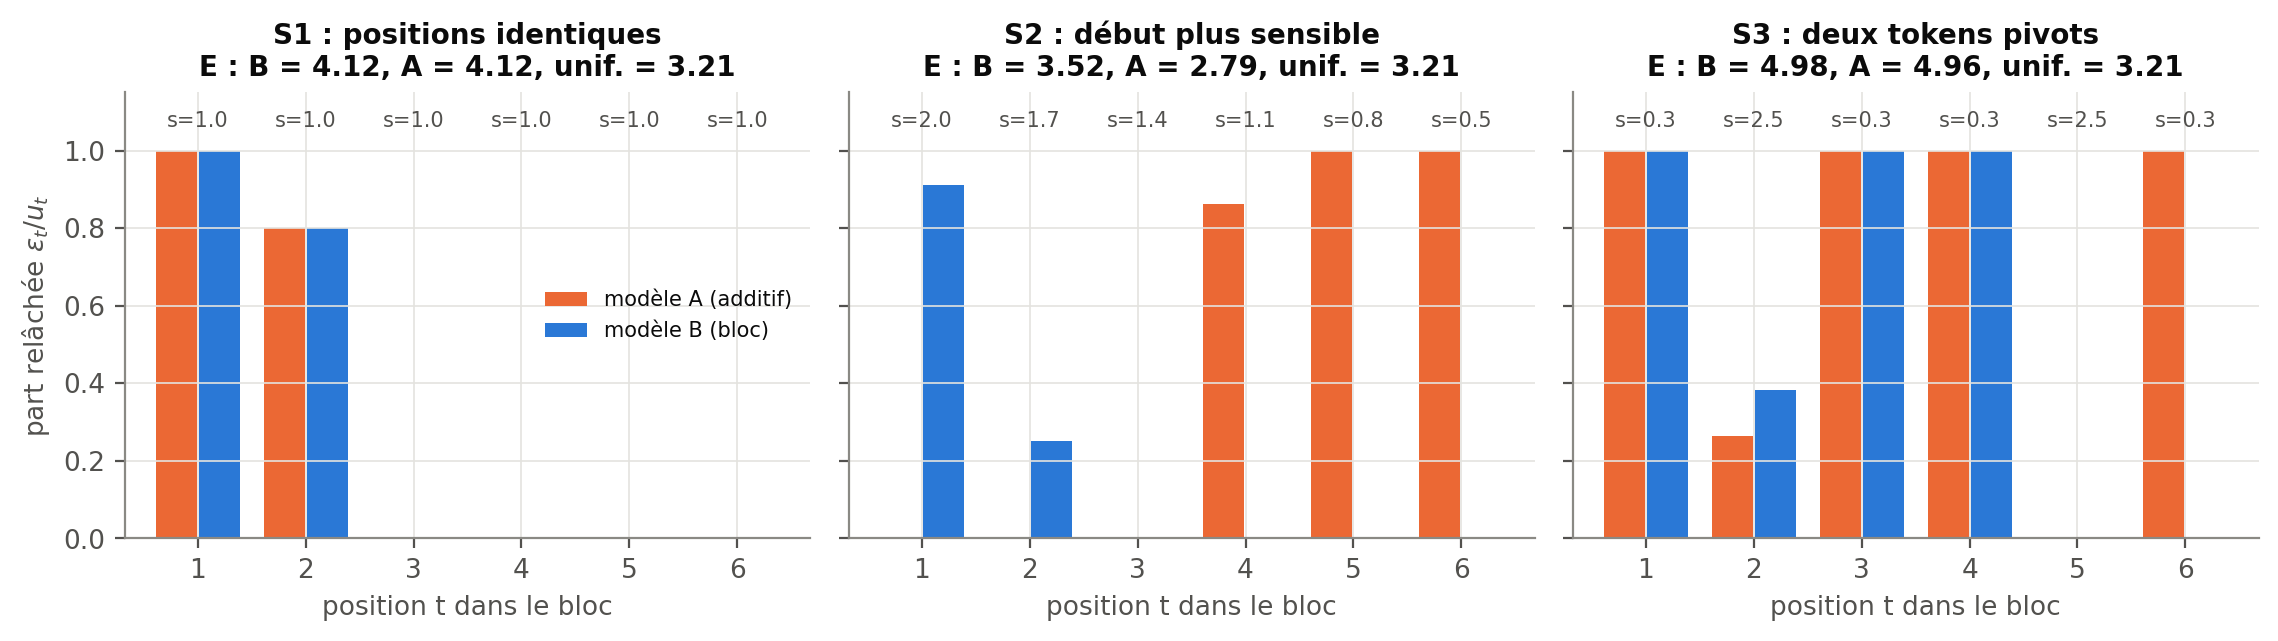
\includegraphics[width=0.9\linewidth]{fig5_allocation.png}
\caption{Part relâchée $\varepsilon_t/u_t$ par position, pour le modèle additif A (orange) et le modèle par blocs B (bleu) ; les sensibilités $s_t$ sont indiquées au-dessus des positions.}
\label{fig:allocation}
\end{figure}

\paragraph{Frontière vitesse--budget (figure~\ref{fig:frontiere}).} En S2, l'optimum gagne jusqu'à 0,97 token par passe sur A et 0,40 sur la déviation uniforme ; l'heuristique « fin d'abord », qui vérifie plus strictement le début comme~\cite{secure} pour la sécurité, est toujours la plus lente. La forme de $E^*(B)$ dépend du profil : convexe en S2, où la complémentarité pousse à concentrer la déviation sur les deux premières positions ; essentiellement concave en S3, où l'on dépense d'abord sur les positions bon marché, puis sur les pivots, comme dans un sac à dos.
L'encadrement~\eqref{eq:encadrement} explique ces deux formes. Pour $B<s\cdot u$, le budget est saturé ; si $B$ n'est pas l'une des valeurs « sommets » $B_I=\sum_{t\in I}s_tu_t$ ($I\subset\{1,\dots,\gamma\}$), l'optimum n'est pas un sommet du pavé, donc il a une position intérieure, et \eqref{eq:encadrement} donne une droite d'appui locale de pente $\lambda$ sous $E^*$. Une fonction continue qui a une telle droite en tout point d'un intervalle y est convexe\footnote{Sinon, $E^*$ moins une de ses cordes atteindrait un maximum $>0$ en un point intérieur ; la droite d'appui y aurait la pente de la corde, et l'ensemble des points de maximum serait ouvert et fermé sans être tout l'intervalle, ce qui contredit la connexité. $E^*$ est continue : si $\varepsilon'$ est optimal pour $B'>B>0$, $(B/B')\varepsilon'$ est admissible pour $B$.}. Ainsi, \textbf{$E^*$ est convexe entre deux valeurs $B_I$ consécutives, et sa pente ne peut baisser qu'en un $B_I$} : en S3, elle chute en $B_I$ pour $I=\{1\}$, $\{1,3\}$, $\{1,3,4\}$ et $\{1,2,3,4,6\}$, à chaque fois qu'une position est saturée.

\begin{figure}[htbp]
\centering
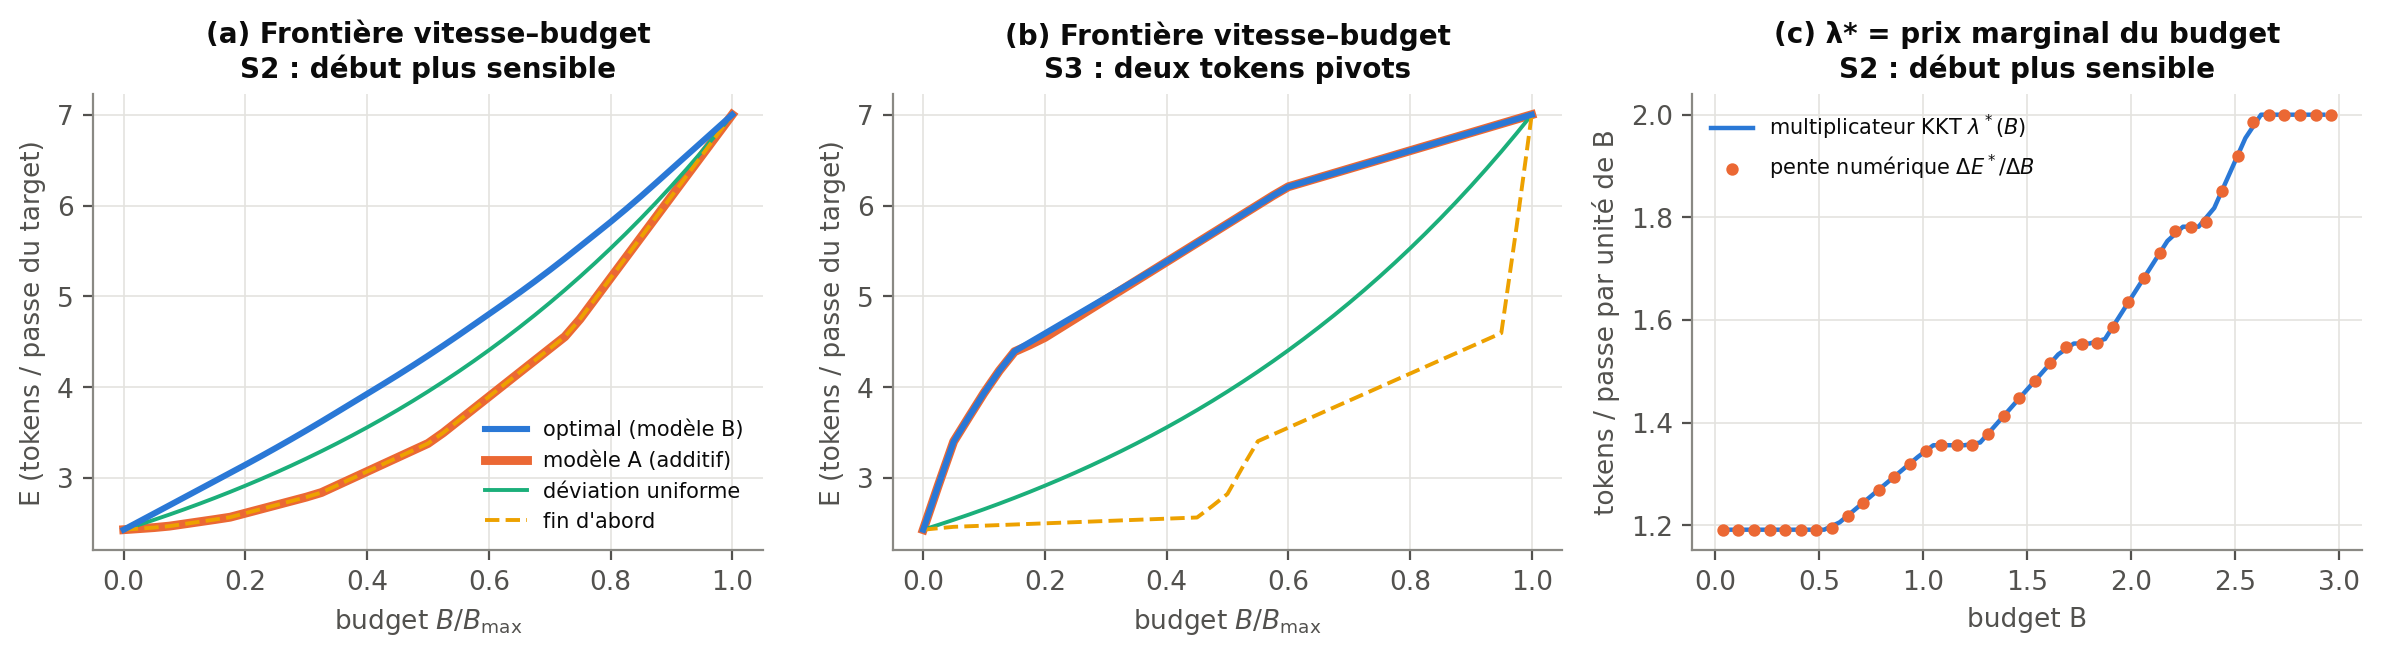
\includegraphics[width=0.94\linewidth]{fig6_frontier.png}
\caption{(a-b) Tokens par passe en fonction du budget, pour l'optimum et trois heuristiques. (c) Multiplicateur KKT $\lambda^*(B)$ et pente numérique $\Delta E^*/\Delta B$ en S2 : $\lambda$ est bien le prix marginal du budget.}
\label{fig:frontiere}
\end{figure}

%=====================================================================
\section{Données réelles et conclusion}\label{sec:reel}
%=====================================================================
\paragraph{Données réelles.} Le target (Qwen2.5-1.5B) rédige des solutions à 16 problèmes GSM8K (2344 tokens) ; à chaque position, on calcule $a_t=\beta(p_t,q_t)$ sur le vocabulaire complet, avec le draft Qwen2.5-0.5B. L'acceptation exacte moyenne vaut 0,893 (0,982 sur les tokens contenant un chiffre). Les sensibilités n'étant pas mesurées dans ce DM, on prend le proxy $s_t=10$ pour les tokens contenant un chiffre et $s_t=1$ sinon, et l'on optimise des blocs de $\gamma=5$ sous un budget commun. À $B=0{,}2\,B_{\max}$, on obtient 5,18 tokens par passe (optimum), contre 4,98 (modèle A) et 4,87 (uniforme). L'optimum relâche la première position du bloc à 73\,\% de sa marge, la deuxième à 43\,\% et les suivantes à 0\,\%, là où A répartit uniformément (22 à 28\,\%) : on retrouve sur données réelles que la déviation doit aller au \textbf{début} du bloc.

\paragraph{Conclusion.} Les deux problèmes se traitent avec les outils du cours. La partie I est un PL de transport : le simplexe et la dualité en donnent la valeur ($1-\TV$), un certificat explicite et le prix exact d'une unité de déviation. La partie II est un problème non concave sous contraintes affines : les contraintes sont qualifiées, les conditions KKT donnent une règle de seuil dont le seuil $\lambda$ est le prix marginal exact du budget, et le gradient projeté converge vers un point KKT, le même depuis tous nos départs. Pour notre projet de recherche, \textbf{la structure en bloc change la réponse} : une règle qui relâche les tokens peu sensibles sans tenir compte de leur position peut perdre plus d'un cinquième de la vitesse atteignable, et la vitesse pousse à relâcher le début du bloc, à l'opposé des heuristiques de sécurité~\cite{secure}.
\textbf{Limites :} (H1) ignore la corrélation entre positions, (H2) est une approximation au premier ordre, les blocs réels se recalent après chaque rejet, et nos sensibilités sont des hypothèses, que le projet devra mesurer.

%=====================================================================
\appendix
\section{Convergence du gradient projeté (cas non concave)}\label{app:convergence}
%=====================================================================
Notons $g=\nabla E(\varepsilon_k)$, $\varepsilon^+=\varepsilon_{k+1}=P_K(\varepsilon_k+\tau g)$, $d=\varepsilon^+-\varepsilon_k$, et $0<\tau<2/L$.
\begin{enumerate}
\item \textbf{Projection.} $P_K(y)$ minimise la fonction convexe $\tfrac12\nr{z-y}^2$ sur le convexe $K$ ; l'inéquation d'Euler (Th.~2.5.1), nécessaire et ici suffisante, donne
\begin{equation*}\label{eq:A1}
z^*=P_K(y)\iff z^*\in K\ \text{ et }\ \sca{z^*-y}{w-z^*}\ge0\quad\forall w\in K.\tag{A.1}
\end{equation*}
Avec $y=\varepsilon_k+\tau g$, $z^*=\varepsilon^+$ et $w=\varepsilon_k$ : $\sca{d-\tau g}{-d}\ge0$, soit $\sca{g}{d}\ge\nr{d}^2/\tau$.
\item \textbf{Montée.} Sur le segment $[\varepsilon_k,\varepsilon^+]\subset K$, $\nabla E$ est $L$-lipschitzien ; par Taylor avec reste intégral, $E(\varepsilon^+)\ge E(\varepsilon_k)+\sca{g}{d}-\frac L2\nr{d}^2$, d'où
\begin{equation*}\label{eq:A3}
E(\varepsilon_{k+1})\ \ge\ E(\varepsilon_k)+\Big(\frac1\tau-\frac L2\Big)\nr{\varepsilon_{k+1}-\varepsilon_k}^2,\qquad \frac1\tau-\frac L2>0.\tag{A.2}
\end{equation*}
\item \textbf{Conséquences.} $E(\varepsilon_k)$ croît et reste majorée par $1+\gamma$ ; en sommant \eqref{eq:A3}, $\sum_k\nr{\varepsilon_{k+1}-\varepsilon_k}^2<\infty$, donc $\nr{\varepsilon_{k+1}-\varepsilon_k}\to0$. $K$ étant compact, une sous-suite $\varepsilon_{k_j}$ converge vers $\bar\varepsilon$, ainsi que $\varepsilon_{k_j+1}$ ; par continuité de $P_K$ (1-lipschitzienne) et de $\nabla E$, $\bar\varepsilon=P_K\big(\bar\varepsilon+\tau\nabla E(\bar\varepsilon)\big)$.
\item \textbf{Point fixe $\iff$ Euler $\iff$ KKT.} Par \eqref{eq:A1}, ce point fixe équivaut à $\sca{\nabla E(\bar\varepsilon)}{w-\bar\varepsilon}\le0$ pour tout $w\in K$ : la condition nécessaire d'Euler pour un minimum local de $J=-E$ sur $K$, équivalente aux conditions KKT du §\ref{sec:kkt} puisque les contraintes sont affines (lemme de Farkas).
\end{enumerate}
Rien ne garantit que $\bar\varepsilon$ soit le maximum \emph{global}, ni que toute la suite converge (c'est le cas si les points KKT sont isolés) : d'où les multi-départs du §\ref{sec:algoII}.

\begin{thebibliography}{9}\small
\bibitem{leviathan} Y.~Leviathan, M.~Kalman, Y.~Matias. \emph{Fast Inference from Transformers via Speculative Decoding}. ICML 2023.
\bibitem{chen} C.~Chen et al. \emph{Accelerating Large Language Model Decoding with Speculative Sampling}. {\NoAutoSpacing arXiv:2302.01318}, 2023.
\bibitem{yin} M.~Yin, M.~Chen, K.~Huang, M.~Wang. \emph{A Theoretical Perspective for Speculative Decoding Algorithm}. NeurIPS 2024.
\bibitem{fuzzy} M.~Holsman, Y.~Huang, B.~Dhingra. \emph{Fuzzy Speculative Decoding for a Tunable Accuracy-Runtime Tradeoff}. Findings of ACL 2025.
\bibitem{secure} Y.~Zhang, Z.~Wang, N.~Gong, Y.~Yang. \emph{Secure Speculative Decoding for Large Language Models}. {\NoAutoSpacing arXiv:2610.08678}, 2026.
\bibitem{allaire} G.~Allaire. \emph{Analyse numérique et optimisation}. Éditions de l'École polytechnique (numérotation des théorèmes reprise du cours).
\end{thebibliography}
\end{document}
